\subsection{Nociones Básicas}
Los \textit{grafos} son estructuras compuestas por \textbf{vértices} y \textbf{aristas}, si el grafo es simple, tienen una propiedad respecto a las aristas, que están formadas por \underline{pares no ordenados} de vértices.
\par Los podemos representar así:
\[
        \mathcal{G} = \left\{\mathcal{V},\mathcal{A}\right\} \left\{\begin{matrix}
                \left\{1,2,3,4,5,6\right\} \\ \left\{ \left\{1,2\right\}, \left\{1,3\right\},  \left\{1,5\right\}, \left\{1,6\right\}, \left\{2,4\right\}, \left\{2,6\right\}, \left\{3,4\right\}, \left\{3,5\right\}\right\}
        \end{matrix}\right.
\]
\begin{minipage}{.6\textwidth}
        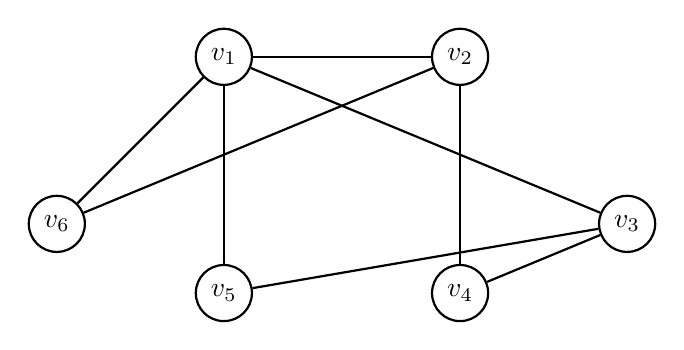
\begin{tikzpicture}[node distance={3cm}, thick, main/.style = {draw, circle}]
                \node[main] (1) {$v_1$};
                \node[main] (2) [right of=1] {$v_2$};
                \node[main] (3) [below right of=2] {$v_3$};
                \node[main] (4) [below of=2] {$v_4$};
                \node[main] (5) [below of=1] {$v_5$};
                \node[main] (6) [below left of=1] {$v_6$};
                \draw (1) -- (2);
                \draw (1) -- (3);
                \draw (1) -- (5);
                \draw (1) -- (6);
                \draw (2) -- (4);
                \draw (2) -- (6);
                \draw (3) -- (4);
                \draw (3) -- (5);
        \end{tikzpicture}
        \par \hspace{4em} \textbf{Representación Gráfica}
\end{minipage}
\begin{minipage}{.6\textwidth}
        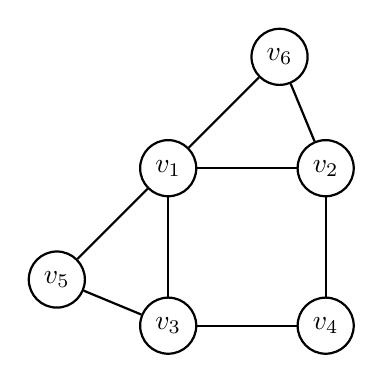
\begin{tikzpicture}[node distance={2cm}, thick, main/.style = {draw, circle}]
                \node[main] (1) {$v_1$};
                \node[main] (2) [right of=1] {$v_2$};
                \node[main] (3) [below of=1] {$v_3$};
                \node[main] (4) [below of=2] {$v_4$};
                \node[main] (5) [below left of=1] {$v_5$};
                \node[main] (6) [above right of=1] {$v_6$};
                \draw (1) -- (2);
                \draw (1) -- (3);
                \draw (1) -- (5);
                \draw (1) -- (6);
                \draw (2) -- (4);
                \draw (2) -- (6);
                \draw (3) -- (4);
                \draw (3) -- (5);
        \end{tikzpicture}
        \par \hspace{4em}\textbf{Grafo Plano}
\end{minipage}
\par \vspace{1em}
La figura de la derecha es su representación gráfica, de la fórmula, mientras que la figura contigua es un \textit{grafo plano}, cuya representación gráfica no posee aristas que se crucen entre si.
\subsubsection{Tipos de Grafos}

\par \textbf{Simple}: Un grafo cuyos vertices están conectados por una única arista, y no se unen a si mismos.
\par  \textbf{Multigrafo}: Grafos cuyos vértices pueden poseer una o más aristas que conecten al mismo vértice:
\par
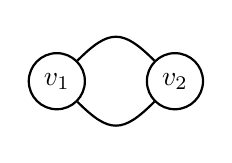
\begin{tikzpicture}[node distance={1.5cm}, thick, main/.style = {draw, circle}]
        \node[main] (1) {$v_1$};
        \node[main] (2) [right of=1] {$v_2$};
        \draw (1) to [out=45,in=135,looseness=1.5] (2);
        \draw (2) to [out=225,in=315,looseness=1.5] (1);
\end{tikzpicture}
\par  \textbf{Pseudografo}: Tipo de multigrafo, que posee aristas que conectan a un vértice consigo mismo:
\par
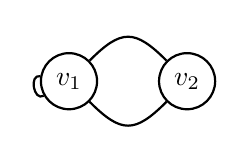
\begin{tikzpicture}[node distance={1.5cm}, thick, main/.style = {draw, circle}]
        \node[main] (1) {$v_1$};
        \node[main] (2) [right of=1] {$v_2$};
        \draw (1) to [out=45,in=135,looseness=1.5] (2);
        \draw (2) to [out=225,in=315,looseness=1.5] (1);
        \draw (1) to [out=170, in= 210, looseness=1.5 ] (1);
\end{tikzpicture}
\par  \textbf{Digrafo} o dirigido: Grafo cuyas aristas tienen un sentido, puede ser:
\begin{itemize}
        \item \underline{Digrafo}, refiriendose a un grafo simple.
        \item \underline{Digrafo Múltiple} o multigrafo dirigido.
        \item \underline{Pseudo Digrafo} o pseudografo dirigido.
\end{itemize} \par
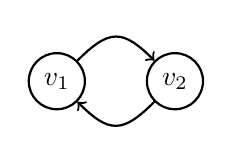
\begin{tikzpicture}[node distance={1.5cm}, thick, main/.style = {draw, circle}]
        \node[main] (1) {$v_1$};
        \node[main] (2) [right of=1] {$v_2$};
        \draw[->](1) to [out=45,in=135,looseness=1.5] (2);
        \draw[->](2) to [out=225,in=315,looseness=1.5] (1);
\end{tikzpicture}
\par  \textbf{Ponderado}: Grafo cuyas aristas poseen un peso:
\par
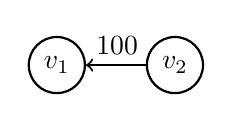
\begin{tikzpicture}[node distance={1.5cm}, thick, main/.style = {draw, circle}]
        \node[main] (1) {$v_1$};
        \node[main] (2) [right of=1] {$v_2$};
        \draw[->] (2) -- node[midway, above right, sloped, pos=1, out=225,in=315,looseness=1.5] {100} (1);
\end{tikzpicture}
\subsubsection{Adyacencia}
Decimos que dos vértices son adyacentes cuando poseen una arista que los conecta directamente. Si miramos el grafo del principio del tema, podemos decir que, el vértice \(v_1\) es adyacente al vértice \(v_5\) pero no al vértice \(v_4\):
\[
        v_i, v_j \in \mathcal{V} \Leftrightarrow e = \left\{v_i,v_j\right\} \in \mathcal{A}
\]
Sabiendo esto, podemos también decir que las aristas que conectan con el mismo vértice, se llaman \textit{incidentes}. Por ejemplo \(\left\{1,3\right\} \) y \(\left\{4,3\right\} \) son incidentes sobre el vértice \(v_3\) pero no lo serán sobre el vértice \(v_6\).
\par Con todo esto, podemos definir entonces que el \textbf{grado} o \textbf{valencia} de un vértice  es el número de aristas que inciden sobre este:
\[
        \delta(v_k) = n
\]
En función del valor de la valencia podemos catalogar al vértice como:
\begin{itemize}
        \item \underline{Vértice Par}, valencia par.
        \item \underline{Vértice Impar}, valencia impar.
        \item \underline{Vértice Aislado}, no tiene valencias.
\end{itemize}
Poseen ciertas características, pero estas pertenecen a los grafos simples, para esto usaremos la siguiente nomenclatura: \(\mathcal{G} = \left\{\mathcal{V},\mathcal{A}\right\}\) será el grafo y \(n = \left\lvert \mathcal{V}\right\rvert \) será la cardinalidad del conjunto de vértices.
\begin{itemize}
        \item Un vértice puede poseer un grado entre 0 y \(n-1\)
        \item Un grafo \(\mathcal{G}\) no puede poseer simultaneamente un vértice de valencia 0 y otro de valencia \(n-1\)
        \item \(\sum_{v \in \mathcal{V}} \delta(v) = 2 \left\lvert A\right\rvert \) es decir, la suma de todas las valencias debe de ser el doble del número de aristas, y por tanto no puede tener un número impar de vértices con una valencia total impar.
\end{itemize}
\subsubsection{Secuencia Gráfica}
Llamaremos a una secuencia gráfica a la lista decreciente de las valencias de todos los vértices del grafo, por ejemplo: \par
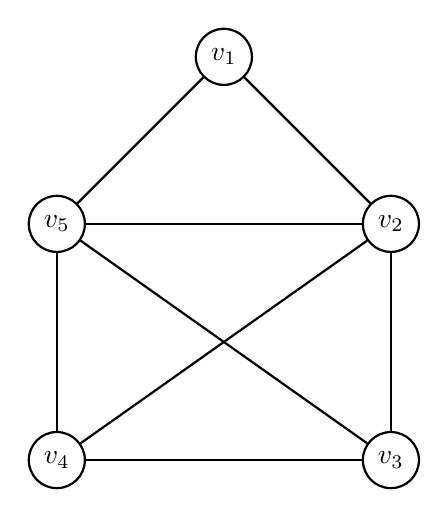
\begin{tikzpicture}[node distance={3cm}, thick, main/.style = {draw, circle}]
        \node[main] (1) {$v_1$};
        \node[main] (2) [below right of=1] {$v_2$};
        \node[main] (3) [below  of=2] {$v_3$};
        \node[main] (5) [below left of=1] {$v_5$};
        \node[main] (4) [below  of=5] {$v_4$};
        \draw (1) -- (2);
        \draw (1) -- (5);
        \draw (5) -- (2);
        \draw (5) -- (4);
        \draw (4) -- (2);
        \draw (4) -- (3);
        \draw (3) -- (2);
        \draw (3) -- (5);
\end{tikzpicture}
\[
        \text{SG} = \left\{4,4,3,3,2\right\}
\]
Con una secuencia gráfica, podemos ser capaces de definir si con esas valencias podemos construir un gráfo, a partir del teorema de Havel-Hakimi.
\subsubsection{Havel-Hakimi}
Este teorema dice dada una secuengia gráfica, con el primer término mayor que cero, es equivalente a:
\begin{enumerate}
        \item Eliminar el primer término, \(a_1\).
        \item Restarle 1 a los \(a_1\) primeros elementos.
        \item Ordenarla decrecientemente
        \item Continuar hasta que \(a_1\) sea menor que 1.
\end{enumerate}
Por ejemplo, dada la SG\(=\left\{1,2,2,3,4\right\} \):
\begin{enumerate}
        \item SG\(=\left\{4,3,2,2,1\right\}\)
        \item SG\(=\left\{3,2,2,1\right\}\)
        \item SG\(=\left\{2,1,1,0\right\}\)
        \item SG\(=\left\{1,1,0\right\}\)
        \item SG\(=\left\{0,0,0\right\}\)
\end{enumerate}
Sabiendo que esta combinación es posible, podemos construir un grafo, llendo de la última a la primera operación, creando tantos vértices como valores vayan apareciendo, cada vértice tendrá un número de aristas que se determinará por el valor que hemos ido decrementando: \par
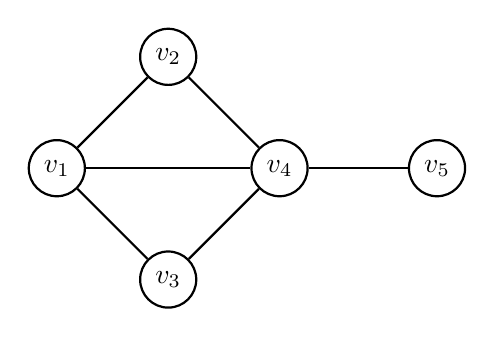
\begin{tikzpicture}[node distance={2cm}, thick, main/.style = {draw, circle}]
        \node[main] (1) {$v_1$};
        \node[main] (2) [above right of=1] {$v_2$};
        \node[main] (3) [below right of=1] {$v_3$};
        \node[main] (4) [below right of=2] {$v_4$};
        \node[main] (5) [right of=4] {$v_5$};
        \draw (1) -- (2);
        \draw (1) -- (3);
        \draw (1) -- (4);
        \draw (4) -- (5);
        \draw (5) -- (4);
        \draw (4) -- (2);
        \draw (4) -- (3);
        \draw (4) -- (1);
\end{tikzpicture}
Si \(a_1\) es menor que cero en algún momento, esa estructura nunca será posible. Tampoco si el \textbf{número de vértices impar es impar} y \textbf{existe un número impar de valencia impar}, o si \(a_1\) \textbf{es mayor que el número total de vértices}.
\subsubsection{Adyacencia en Digrafos}
Simplemente tenemos que tener en cuenta, que en este tipo de grafos, debemos de separar las valencias de las aristas que \textbf{entran} y de las que \textbf{salen}.
\subsubsection{Grafos Especiales}
\textbf{Grafos Triviales}: No poseen aristas. \par
\textbf{Sin ciclos}: Grafos que no están cerrados, no puedes llegar a un vértice desde si mismo. Pueden ser:
\par \hspace{1em} \textbf{\textit{Árbol}}: \par
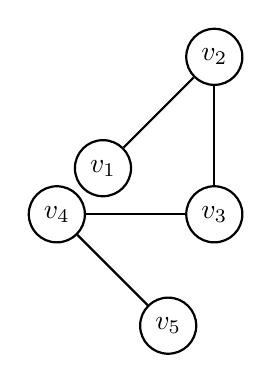
\begin{tikzpicture}[node distance={2cm}, thick, main/.style = {draw, circle}]
        \node[main] (1) {$v_1$};
        \node[main] (2) [above right of=1] {$v_2$};
        \node[main] (3) [below of=2] {$v_3$};
        \node[main] (4) [left of=3] {$v_4$};
        \node[main] (5) [below right of=4] {$v_5$};
        \draw (1) -- (2);
        \draw (2) -- (3);
        \draw (3) -- (4);
        \draw (4) -- (5);
\end{tikzpicture}
\par \hspace{1em} \textbf{\textit{Bosque de Árboles}}: \par
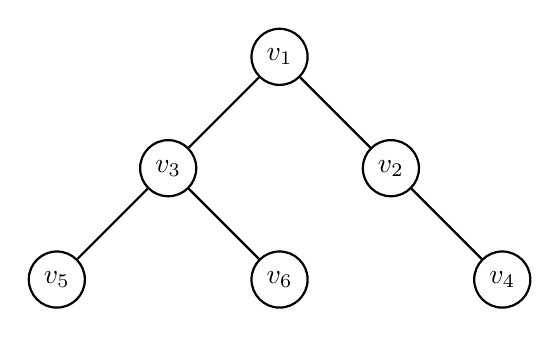
\begin{tikzpicture}[node distance={2cm}, thick, main/.style = {draw, circle}]
        \node[main] (1) {$v_1$};
        \node[main] (2) [below right of=1] {$v_2$};
        \node[main] (3) [below left of=1] {$v_3$};
        \node[main] (4) [below right of=2] {$v_4$};
        \node[main] (5) [below left of=3] {$v_5$};
        \node[main] (6) [below right of=3] {$v_6$};
        \draw (1) -- (2);
        \draw (1) -- (3);
        \draw (2) -- (4);
        \draw (3) -- (5);
        \draw (3) -- (6);
\end{tikzpicture}
\par \textbf{Con ciclos}:
\par \hspace{1em} \textbf{\textit{Grafo Ciclo}} \(C_n\).
\par \hspace{1em} \textbf{\textit{Grafo Completo}} \(K_n\), todos los vértices tienen la máxima valencia posible.
\par \hspace{1em} \textbf{\textit{Grafo Regular}}: Todos los vértices tienen el mismo número de valencia.
\par \textbf{Grafo Bipartito}: Por definición, son aquellos grafos que pueden formarse a partir de dos conjuntos de vértices, que no comparten ningún vértice en común (es decir, son grafos \textbf{disjuntos}):
\[
        \mathcal{G} = \left\{\mathcal{V},\mathcal{A}\right\} \left\{\begin{matrix}
                \mathcal{V} = \mathcal{V}_1 \cup \mathcal{V}_2, \mathcal{V}_1 \cap  \mathcal{V}_2 = \emptyset
                \\
                \forall_e \in \mathcal{A}: e = \left \{ v_i, v_j \right \}, v_1 \in \mathcal{V}_1, v_2 \in \mathcal{V}_2
        \end{matrix}\right.
\]
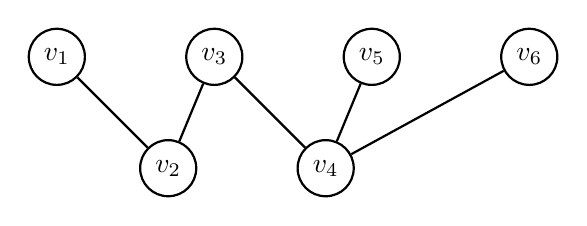
\begin{tikzpicture}[node distance={2cm}, thick, main/.style = {draw, circle}]
        \node[main] (1) {$v_1$};
        \node[main] (3) [right of=1] {$v_3$};
        \node[main] (5) [right of=3] {$v_5$};
        \node[main] (6) [right of=5] {$v_6$};
        \node[main] (4) [below right of=3] {$v_4$};
        \node[main] (2) [below right of=1] {$v_2$};
        \draw (1) -- (2);
        \draw (2) -- (3);
        \draw (3) -- (4);
        \draw (4) -- (5);
        \draw (4) -- (6);
\end{tikzpicture}
\par \textbf{Grafo Bipartito Completo} \(K_{n,m}\): Son grafos que cumplen la condición de ser bipartito, y además todos sus vértices tienen valencia máxima. \par
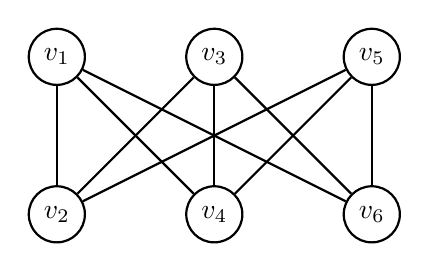
\begin{tikzpicture}[node distance={2cm}, thick, main/.style = {draw, circle}]
        \node[main] (1) {$v_1$};
        \node[main] (3) [right of=1] {$v_3$};
        \node[main] (5) [right of=3] {$v_5$};
        \node[main] (2) [below of=1] {$v_2$};
        \node[main] (4) [right of=2] {$v_4$};
        \node[main] (6) [right of=4] {$v_6$};
        \draw (1) -- (2);
        \draw (1) -- (4);
        \draw (1) -- (6);
        \draw (3) -- (2);
        \draw (3) -- (4);
        \draw (3) -- (6);
        \draw (5) -- (2);
        \draw (5) -- (6);
        \draw (5) -- (4);

\end{tikzpicture}
\subsection{Sugrafos}
No es más que un subconjunto de \(\mathcal{V}\) y \(\mathcal{A}\) que nos permite obtener otro nuevo grafo:
\[
        \mathcal{G}' \subseteq \mathcal{G} \Leftrightarrow \left\{\begin{matrix}
                \mathcal{V}' \subseteq \mathcal{V}
                \\
                \mathcal{A}' \subseteq \mathcal{A}
        \end{matrix}\right.
\]
\begin{minipage}{.6\textwidth}
        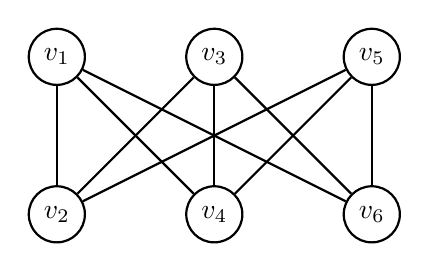
\begin{tikzpicture}[node distance={2cm}, thick, main/.style = {draw, circle}]
                \node[main] (1) {$v_1$};
                \node[main] (3) [right of=1] {$v_3$};
                \node[main] (5) [right of=3] {$v_5$};
                \node[main] (2) [below of=1] {$v_2$};
                \node[main] (4) [right of=2] {$v_4$};
                \node[main] (6) [right of=4] {$v_6$};
                \draw (1) -- (2);
                \draw (1) -- (4);
                \draw (1) -- (6);
                \draw (3) -- (2);
                \draw (3) -- (4);
                \draw (3) -- (6);
                \draw (5) -- (2);
                \draw (5) -- (6);
                \draw (5) -- (4);

        \end{tikzpicture}
        \par \hspace{6em}\(\mathcal{G}\)
\end{minipage}
\begin{minipage}{.6\textwidth}
        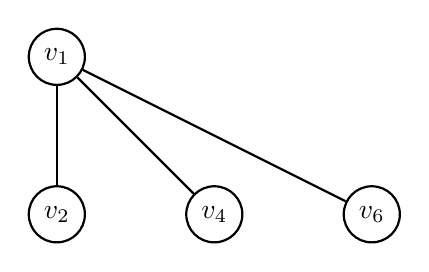
\begin{tikzpicture}[node distance={2cm}, thick, main/.style = {draw, circle}]
                \node[main] (1) {$v_1$};
                \node[main] (2) [below of=1] {$v_2$};
                \node[main] (4) [right of=2] {$v_4$};
                \node[main] (6) [right of=4] {$v_6$};
                \draw (1) -- (2);
                \draw (1) -- (4);
                \draw (1) -- (6);
        \end{tikzpicture}
        \par \hspace{6em}\(\mathcal{G}'\)
\end{minipage}
Podemos obtener un subgrafo a partir de un conjunto de vértices, o aristas, u ambas (en cualquier caso, también deberemos de obtener los vértices y aristas que pertenezcan a esa arísta u vertice).
\subsubsection{Subgrafo especial}
Un subgrafo especial es el \textit{subgrafo recubrido}, el cual se genera cuando solo generamos un subgrafo con \textbf{todos} los vértices del grafo original, obteniendo la menor cantidad de aristas
\subsection{Operaciones con Grafos}
Solo podemos hacer 5 operaciones con grafos:
\begin{itemize}
        \item \textbf{Eliminación de Aristas}: Eliminar una arista, no implica borrar sus vértices.
        \item \textbf{Eliminación de Vértices}: Si eliminamos un vértice, borramos cualquier arista que se conecte a este.
        \item \textbf{Unión de Grafos}: \par

              \begin{minipage}{.2\textwidth}
                      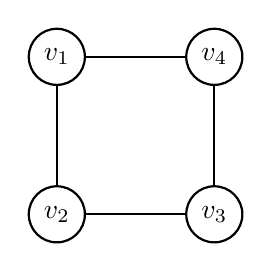
\begin{tikzpicture}[node distance={2cm}, thick, main/.style = {draw, circle}]
                              \node[main] (1) {$v_1$};
                              \node[main] (2) [below of=1] {$v_2$};
                              \node[main] (3) [right of=2] {$v_3$};
                              \node[main] (4) [above of=3] {$v_4$};
                              \draw (1) -- (2);
                              \draw (2) -- (3);
                              \draw (3) -- (4);
                              \draw (4) --(1);
                      \end{tikzpicture}
              \end{minipage}
              \(\bigcup \)
              \begin{minipage}{.2\textwidth}
                      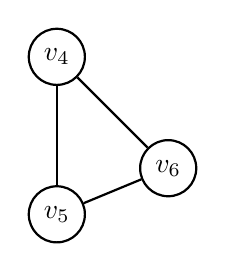
\begin{tikzpicture}[node distance={2cm}, thick, main/.style = {draw, circle}]
                              \node[main] (4) {$v_4$};
                              \node[main] (5) [below of=4] {$v_5$};
                              \node[main] (6) [below right of=4] {$v_6$};
                              \draw (4) -- (5); \draw (6) -- (4); \draw (6) -- (5);

                      \end{tikzpicture}
              \end{minipage}
              \(=\)
              \begin{minipage}{.1\textwidth}
                      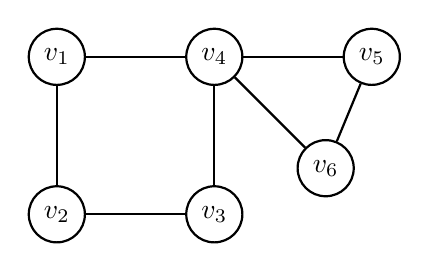
\begin{tikzpicture}[node distance={2cm}, thick, main/.style = {draw, circle}]
                              \node[main] (1) {$v_1$};
                              \node[main] (2) [below of=1] {$v_2$};
                              \node[main] (3) [right of=2] {$v_3$};
                              \node[main] (4) [above of=3] {$v_4$};
                              \draw (1) -- (2);
                              \draw (2) -- (3);
                              \draw (3) -- (4);
                              \draw (4) --(1);
                              \node[main] (5) [right of=4] {$v_5$};
                              \node[main] (6) [below right of=4] {$v_6$};
                              \draw (4) -- (5); \draw (6) -- (4); \draw (6) -- (5);
                      \end{tikzpicture}
              \end{minipage}
        \item \textbf{Intersección de Grafos}: \par

              \begin{minipage}{.2\textwidth}
                      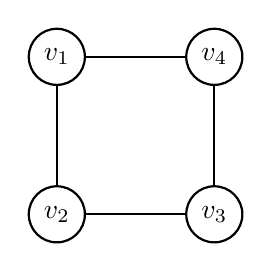
\begin{tikzpicture}[node distance={2cm}, thick, main/.style = {draw, circle}]
                              \node[main] (1) {$v_1$};
                              \node[main] (2) [below of=1] {$v_2$};
                              \node[main] (3) [right of=2] {$v_3$};
                              \node[main] (4) [above of=3] {$v_4$};
                              \draw (1) -- (2);
                              \draw (2) -- (3);
                              \draw (3) -- (4);
                              \draw (4) --(1);
                      \end{tikzpicture}
              \end{minipage}
              \(\bigcap \)
              \begin{minipage}{.2\textwidth}
                      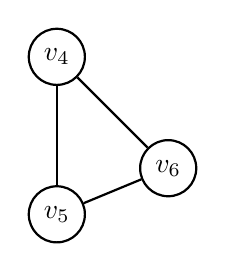
\begin{tikzpicture}[node distance={2cm}, thick, main/.style = {draw, circle}]
                              \node[main] (4) {$v_4$};
                              \node[main] (5) [below of=4] {$v_5$};
                              \node[main] (6) [below right of=4] {$v_6$};
                              \draw (4) -- (5);
                              \draw (6) -- (4);
                              \draw (6) -- (5);
                      \end{tikzpicture}
              \end{minipage}
              \(=\)
              \begin{minipage}{.1\textwidth}
                      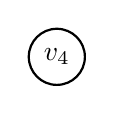
\begin{tikzpicture}[node distance={2cm}, thick, main/.style = {draw, circle}]
                              \node[main] (1) {$v_4$};
                      \end{tikzpicture}
              \end{minipage}
        \item \textbf{Suma de Grafos} (cuando son Disjuntos): Hacemos todas las posibles combinaciones de aristas entre los vértices de los dos grafos, un producto cartesiano:
              \par
              \begin{minipage}{.2\textwidth}
                      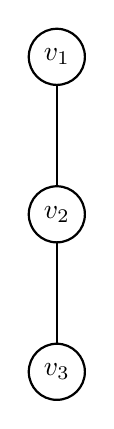
\begin{tikzpicture}[node distance={2cm}, thick, main/.style = {draw, circle}]
                              \node[main] (1) {$v_1$};
                              \node[main] (2) [below of=1] {$v_2$};
                              \node[main] (3) [below of=2] {$v_3$};
                              \draw (1) -- (2);
                              \draw (2) -- (3);
                      \end{tikzpicture}
              \end{minipage}
              \(+\)
              \begin{minipage}{.2\textwidth}
                      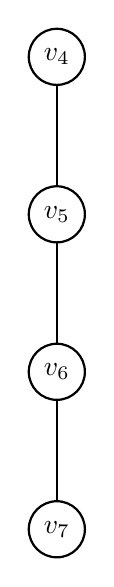
\begin{tikzpicture}[node distance={2cm}, thick, main/.style = {draw, circle}]
                              \node[main] (4) {$v_4$};
                              \node[main] (5) [below of=4] {$v_5$};
                              \node[main] (6) [below of=5] {$v_6$};
                              \node[main] (7) [below of=6] {$v_7$};
                              \draw (4) -- (5);
                              \draw (5) -- (6);
                              \draw (6) -- (7);
                      \end{tikzpicture}
              \end{minipage}
              \(=\)
              \begin{minipage}{.2\textwidth}
                      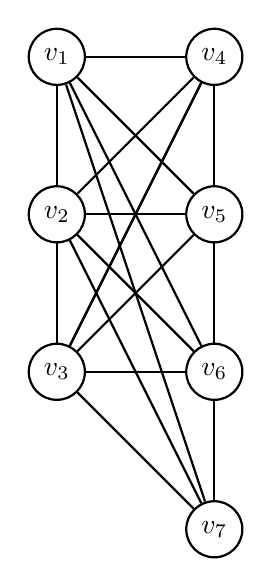
\begin{tikzpicture}[node distance={2cm}, thick, main/.style = {draw, circle}]
                              \node[main] (1) {$v_1$};
                              \node[main] (2) [below of=1] {$v_2$};
                              \node[main] (3) [below of=2] {$v_3$};
                              \node[main] (4) [right of=1]{$v_4$};
                              \node[main] (5) [below of=4] {$v_5$};
                              \node[main] (6) [below of=5] {$v_6$};
                              \node[main] (7) [below of=6] {$v_7$};
                              \draw (1) -- (2);
                              \draw (2) -- (3);
                              \draw (3) -- (4);
                              \draw (4) -- (1);
                              \draw (4) -- (5);
                              \draw (5) -- (6);
                              \draw (6) -- (7);
                              \draw (1) -- (4);
                              \draw (1) -- (5);
                              \draw (1) -- (6);
                              \draw (1) -- (7);
                              \draw (2) -- (4);
                              \draw (3) -- (4);
                              \draw (3) -- (6);
                              \draw (3) -- (5);
                              \draw (3) -- (7);
                              \draw (2) -- (6);
                              \draw (2) -- (5);
                              \draw (2) -- (7);
                      \end{tikzpicture}
              \end{minipage}
\end{itemize}
\subsubsection{Grafo Rueda}
\[
        W_n = K_1 + C_n
\]
Este tipo de grafo se obtiene de la suma de un grafo con un solo vértice, y un circular (tendrémos \(n+1\) vértices) pero lo llamaremos \(W_n\), un ejemplo es el siguiente
\par
\begin{minipage}{.2\textwidth}
        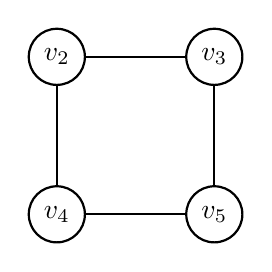
\begin{tikzpicture}[node distance={2cm}, thick, main/.style = {draw, circle}]
                \node[main] (1) {$v_2$};
                \node[main] (2) [right of=1] {$v_3$};
                \node[main] (3) [below of=1] {$v_4$};
                \node[main] (5) [right of=3] {$v_5$};
                \draw (1) -- (2);
                \draw (2) -- (5);
                \draw (3) -- (5);
                \draw (3) -- (1);
        \end{tikzpicture}
\end{minipage}
\(+\)
\begin{minipage}{.2\textwidth}
        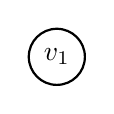
\begin{tikzpicture}[node distance={2cm}, thick, main/.style = {draw, circle}]
                \node[main] (4) {$v_1$};
        \end{tikzpicture}
\end{minipage}
\(=\)
\begin{minipage}{.2\textwidth}
        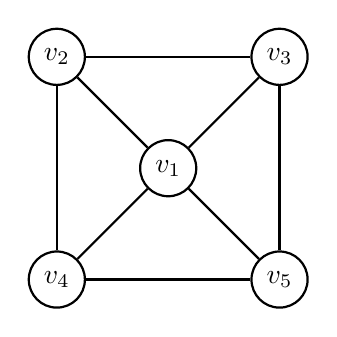
\begin{tikzpicture}[node distance={2cm}, thick, main/.style = {draw, circle}]
                \node[main] (1) {$v_2$};
                \node[main] (4) [below right of= 1]{$v_1$};
                \node[main] (2) [above right of=4] {$v_3$};
                \node[main] (3) [below left of=4] {$v_4$};
                \node[main] (5) [below right of=4] {$v_5$};
                \draw (1) -- (2);
                \draw (2) -- (5);
                \draw (3) -- (5);
                \draw (3) -- (1);
                \draw (4) -- (1);
                \draw (4) -- (2);
                \draw (4) -- (3);
                \draw (4) -- (5);
        \end{tikzpicture}
\end{minipage}
\subsubsection{Grafo Complementario}
Es el grafo resultante de las aristas que no se han creado. \par
\begin{minipage}{.4\textwidth}
        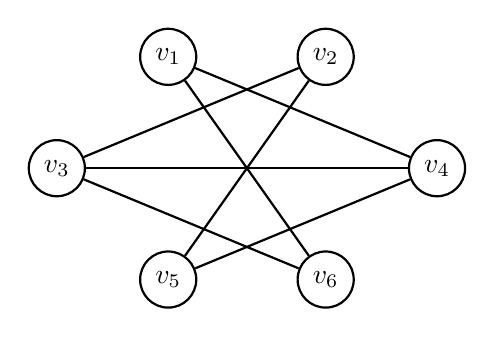
\begin{tikzpicture}[node distance={2cm}, thick, main/.style = {draw, circle}]
                \node[main] (1) {$v_1$};
                \node[main] (2) [right of=1] {$v_2$};
                \node[main] (3) [below left of = 1]{$v_3$};
                \node[main] (4) [below right of = 2]{$v_4$};
                \node[main] (5) [below right of = 3]{$v_5$};
                \node[main] (6) [below left of = 4]{$v_6$};
                \draw (1) -- (4);
                \draw (4) -- (3);
                \draw (3) -- (2);
                \draw (2) -- (5);
                \draw (5) -- (4);
                \draw (3) -- (6);
                \draw (6) -- (1);
        \end{tikzpicture}
        \par \hspace{3.5em}\textbf{Grafo Original} \par \hspace{4em}\(\mathcal{G} =  \left\{\mathcal{V}, \mathcal{A}\right\} \)
\end{minipage}
\begin{minipage}{.4\textwidth}
        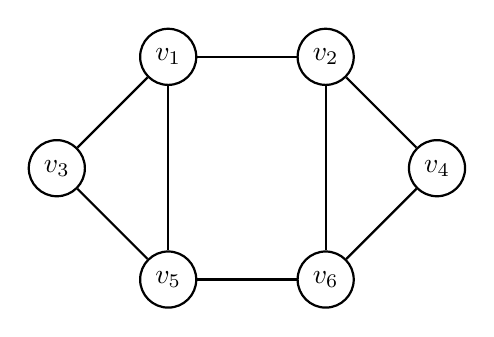
\begin{tikzpicture}[node distance={2cm}, thick, main/.style = {draw, circle}]
                \node[main] (1) {$v_1$};
                \node[main] (2) [right of=1] {$v_2$};
                \node[main] (3) [below left of = 1]{$v_3$};
                \node[main] (4) [below right of = 2]{$v_4$};
                \node[main] (5) [below right of = 3]{$v_5$};
                \node[main] (6) [below left of = 4]{$v_6$};
                \draw (1) -- (2);
                \draw (2) -- (4);
                \draw (4) -- (6);
                \draw (3) -- (5);
                \draw (5) -- (6);
                \draw (3) -- (1);
                \draw (1) -- (5);
                \draw (2) -- (6);
        \end{tikzpicture}
        \par \hspace{2em}\textbf{Grafo Complementario} \par \hspace{4em}\(\overline{\mathcal{G}} =  \left\{\mathcal{V}, \overline{\mathcal{A}}\right\} \)
\end{minipage}
\subsubsection{Grafo de Línea}
Dado un grafo con \(n\) vértices y \(m\) aristas, podemos crear un grafo a partir de las aristas adyacentes, las cuales son aquellas conectadas por un vértice: \par
\begin{minipage}{.4\textwidth}
        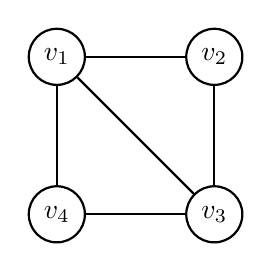
\begin{tikzpicture}[node distance={2cm}, thick, main/.style = {draw, circle}]
                \node[main] (1) {$v_1$};
                \node[main] (2) [right of=1] {$v_2$};
                \node[main] (3) [below  of = 2]{$v_3$};
                \node[main] (4) [below of = 1]{$v_4$};
                \draw (1) -- (2);
                \draw (2) --(3);
                \draw (3) --(4);
                \draw (4) --(1);
                \draw (1) --(3);
        \end{tikzpicture}
        \par \hspace{3.5em}\textbf{Grafo Original}
\end{minipage}
\begin{minipage}{.4\textwidth}
        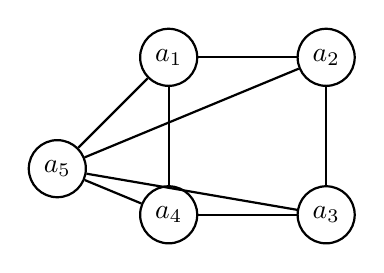
\begin{tikzpicture}[node distance={2cm}, thick, main/.style = {draw, circle}]
                \node[main] (1) {$a_1$};
                \node[main] (2) [right of=1] {$a_2$};
                \node[main] (3) [below  of = 2]{$a_3$};
                \node[main] (4) [below of = 1]{$a_4$};
                \node[main] (5) [below left of = 1]{$a_5$};
                \draw (1) -- (2);
                \draw (1) -- (5);
                \draw (1) -- (4);
                \draw (2) -- (3);
                \draw (3) -- (5);
                \draw (3) -- (4);
                \draw (5) -- (2);
                \draw (5) -- (4);
        \end{tikzpicture}
        \par \hspace{2.5em}\textbf{Grafo de Línea}
\end{minipage}
\subsection{Definir un Grafo}
Existen distintas formas, hasta ahora se ha visto la forma gráfica, sin embargo si el grafo es extremadamente grande es mejor utilizar \textit{listas de adyacencias} o \textit{matrices de adyacencias}:
\begin{itemize}
        \item \textbf{Listas de adyacencias}: Creamos un conjunto de listas, que guardan la información relativa a los vértices que está unido el vértice de esa posición:\[
                      \left\{\left\{2,3,5,6\right\},\left\{1,4,6\right\} , \left\{1,4,5\right\} ,\left\{2,3\right\} , \left\{1,3\right\} , \left\{1,2\right\}\right\}
              \]
        \item \textbf{Matrices de Adyacencias}: Matriz de \(n\)X\(m\) que, dependiendo del tipo de grafo, guardará unos valores u otros:\begin{itemize}
                      \item Si es simple, guardará un \(1\) por cada posición correspondiente en la que el vértice de esa fila, tenga una arista con el vértice de esa columna. \begin{itemize}
                                    \item La suma de las columnas es la valencia.
                                    \item La diagonal es nula.
                                    \item Es cuadrada y simétrica.
                            \end{itemize}
                      \item Si es simple, podemos crear una matriz tal que guarde qué vértice con que otro guarda relación
                            \begin{itemize}
                                    \item La suma de cada columna es 2.
                                    \item La suma de cada fila es la valencia de ese vértice.
                            \end{itemize}
                      \item Si es un digrafo, se hace igual que el simple.\begin{itemize}
                                    \item La suma de cada fila es la valencia saliente.
                                    \item La suma de cada columna es la valencia de entrada.
                            \end{itemize}
                      \item En un pseudografo, en vez de guardar un 1, guardamos el valor de aristas que conectan con ese vértice. Si es circular, sumas le sumas 2.
                      \item Si es ponderado, guardas el peso de la arista en la posición que le corresponde a la relación de los vértices.
              \end{itemize}
\end{itemize}
\subsection{Isomorfismo de Grafos}
Un grafo es isomorfo, cuando cumple la propiedad de ser biyectivo, es decir, es inyectiva (por un vértice del grafo existe una imágen en el adyacente) y es sobreyectiva (para cada vértice del grafo, existe una imágen en el adyacente).
\par
Debemos de tener en cuenta ciertos detalles, si queremos comprobar que no hay isomorfismo:
\begin{enumerate}
        \item El número de vértices debe ser el mismo.
        \item El número de aristas debe de ser el mismo.
        \item Los grados de los vértices, deben de ser los mismos.
        \item El número de ciclos, de igual longitud, deben de ser los mismos.
        \item El número de componentes conexas debe ser igual.
        \item Los grafos complementarios deben de ser Isomorfos
        \item Cada vértice debe de tener una imágen, que cumpla sus propiedades.
        \item ...
\end{enumerate}
Si son isomorfos, debemos de encontrar una aplicación, por la cual podemos decir que un vértice de un grafo, equivale a otro vértice del otro gráfo.
\subsubsection{Grafo Autocomplementario}
Un grafo es autocomplementario, cuando su complementario sufre de Isomorfismo.